% Ahmed body side-view schematic (TikZ)
% All coordinates in mm, scaled by 1/100 so 1 unit = 100 mm.
% Geometry matches generate_ahmed_freecad.py (Lienhart reference):
%   L = 1044 mm, H = 288 mm, h = 50.8 mm, R_nose = 100 mm (top AND bottom front edges)
%   Slant:    starts x = 822 mm, drop = 222*tan(alpha_slant); drawn at 25 deg
%   Diffuser: starts x = 869 mm, rise = 175*tan(alpha_diff);  drawn at 10 deg
%   Slant and diffuser both terminate at the rear face (x = L) — they overlap in x.
%   Legs: cylinders R = 15 mm centred at x = 195 mm and x = 849 mm.

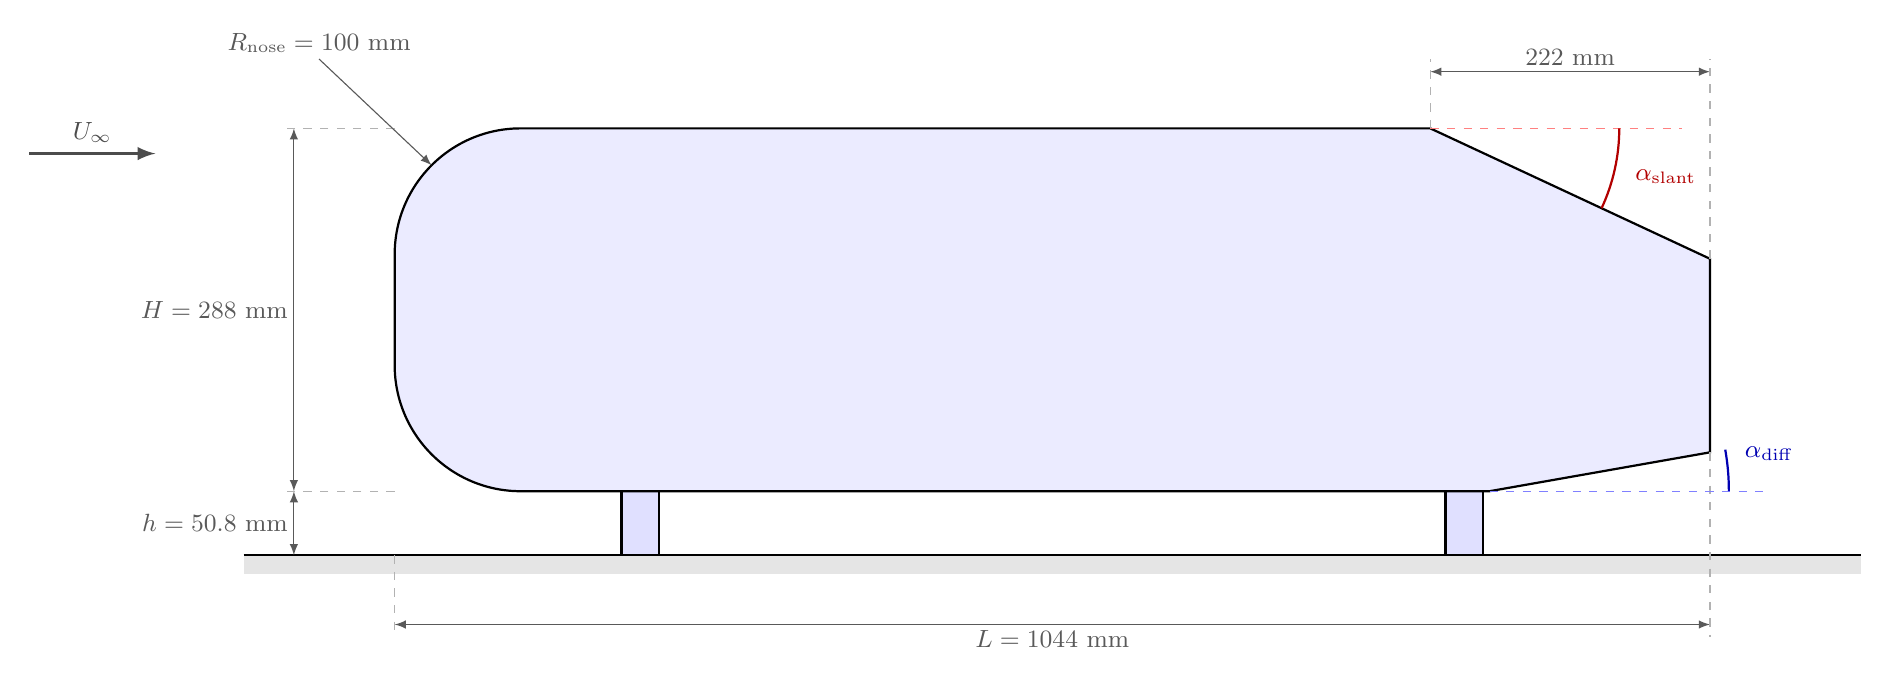
\begin{tikzpicture}[
  scale=1.6,
  >=latex,
  dim/.style={<->, thin, gray!70!black},
  ext/.style={gray!60, thin, dashed},
  dimlbl/.style={font=\small, inner sep=2pt},
  annlbl/.style={font=\small\itshape},
]

% ── Parameters (unit = 100 mm) ────────────────────────────────────────────────
\def\rh{0.508}        % ride height h
\def\H{2.88}          % body height H
\def\L{10.44}         % body length L
\def\R{1.0}           % nose fillet radius R_nose
\def\xslant{8.22}     % slant start (822 mm)
\def\xdiff{8.69}      % diffuser start (869 mm)
\def\slantang{25}     % drawn slant angle (deg)
\def\diffang{10}      % drawn diffuser angle (deg)

% Derived
\pgfmathsetmacro{\yfloor}{\rh}
\pgfmathsetmacro{\yroof}{\rh + \H}
\pgfmathsetmacro{\sdrop}{(\L - \xslant)*tan(\slantang)}   % slant vertical drop
\pgfmathsetmacro{\drise}{(\L - \xdiff)*tan(\diffang)}     % diffuser vertical rise
\pgfmathsetmacro{\yslantend}{\yroof - \sdrop}
\pgfmathsetmacro{\ydiffend}{\yfloor + \drise}

% ── Ground line ───────────────────────────────────────────────────────────────
\fill[gray!20] (-1.2, -0.15) rectangle (\L + 1.2, 0);
\draw[thick] (-1.2, 0) -- (\L + 1.2, 0);

% ── Leg stubs (cylinders R=15 mm at x=195, 849 mm; drawn behind body) ────────
\fill[blue!12, draw=black, thick] (1.80, 0) rectangle (2.10, \yfloor);
\fill[blue!12, draw=black, thick] (8.34, 0) rectangle (8.64, \yfloor);

% ── Body silhouette (single closed path, nose fillets included) ──────────────
\draw[fill=blue!8, thick]
  (\R, \yfloor)                                        % bottom of nose fillet
  -- (\xdiff, \yfloor)                                 % underbody
  -- (\L, \ydiffend)                                   % diffuser ramp
  -- (\L, \yslantend)                                  % rear face (base)
  -- (\xslant, \yroof)                                 % slant
  -- (\R, \yroof)                                      % roof
  arc[start angle=90, end angle=180, radius=\R]        % top nose fillet
  -- (0, \yfloor + \R)                                 % front face
  arc[start angle=180, end angle=270, radius=\R]       % bottom nose fillet
  -- cycle;

% ── Dimension: total length L ─────────────────────────────────────────────────
\draw[dim] (0, -0.55) -- (\L, -0.55)
  node[midway, below, dimlbl] {$L = 1044\ \mathrm{mm}$};
\draw[ext] (0, 0)         -- (0, -0.65);
\draw[ext] (\L, \ydiffend) -- (\L, -0.65);

% ── Dimensions: ride height h, body height H ─────────────────────────────────
\draw[dim] (-0.8, 0) -- (-0.8, \yfloor)
  node[midway, left, dimlbl] {$h = 50.8\ \mathrm{mm}$};
\draw[dim] (-0.8, \yfloor) -- (-0.8, \yroof)
  node[midway, left, dimlbl] {$H = 288\ \mathrm{mm}$};
\draw[ext] (0, \yfloor) -- (-0.9, \yfloor);
\draw[ext] (0, \yroof)  -- (-0.9, \yroof);

% ── Dimension: slant horizontal extent (222 mm) ──────────────────────────────
\draw[dim] (\xslant, \yroof + 0.45) -- (\L, \yroof + 0.45)
  node[midway, above, dimlbl] {$222\ \mathrm{mm}$};
\draw[ext] (\xslant, \yroof)    -- (\xslant, \yroof + 0.55);
\draw[ext] (\L, \yslantend)     -- (\L, \yroof + 0.55);

% ── Nose fillet radius R_nose ─────────────────────────────────────────────────
% Leader from top fillet arc midpoint
\draw[->, thin, gray!70!black]
  (\R - 1.6, \yroof + 0.55) node[above, dimlbl] {$R_\mathrm{nose} = 100\ \mathrm{mm}$}
  -- ({\R - \R*cos(45)}, {\yroof - \R + \R*sin(45)});

% ── Slant angle alpha_slant (design variable) ────────────────────────────────
% Measured at the slant-start corner between the roof extension and the slant.
\draw[ext, red!50] (\xslant, \yroof) -- (\xslant + 2.0, \yroof);
\draw[thick, red!70!black]
  (\xslant + 1.5, \yroof)
  arc[start angle=0, end angle=-\slantang, radius=1.5];
\node[red!70!black, annlbl, right] at (\xslant + 1.55, \yroof - 0.38)
  {$\alpha_\mathrm{slant}$};

% ── Diffuser angle alpha_diff (design variable) ──────────────────────────────
% Measured at the diffuser-start corner between the underbody extension and the ramp.
\draw[ext, blue!50] (\xdiff, \yfloor) -- (\xdiff + 2.2, \yfloor);
\draw[thick, blue!70!black]
  (\xdiff + 1.9, \yfloor)
  arc[start angle=0, end angle=\diffang, radius=1.9];
\node[blue!70!black, annlbl, right] at (\xdiff + 1.95, \yfloor + 0.30)
  {$\alpha_\mathrm{diff}$};

% ── Flow direction arrow ──────────────────────────────────────────────────────
\draw[->, very thick, gray!60!black]
  (-2.9, {\yroof - 0.2}) -- (-1.9, {\yroof - 0.2})
  node[midway, above, font=\small] {$U_\infty$};

\end{tikzpicture}
